In this Chapter, we conducted 4 different evaluations in simple maze environments to investigate how the ILP(RL) agent learns and finds the optimal policy.

\section{Experimental Setup}
\label{sec:experimental_setup}

\subsection{Evaluation Metrics}
\label{subsec:evaluation_metrics}

As introduced in Section \ref{sec:motivation}, our motivation is to improve the learning efficiency and capability of transfer learning in RL.
Therefore, these are the two main measurements for the performance of ILP(RL).
The learning efficiency is measured in three different ways: performance of optimal policy, convergence of inductive learning and runtime of ILP(RL). Due to the random exploration for both ILP(RL) and a benchmark, the performance of each experiment varies. Especially ASP planning of ILP(RL) starts only when the agent finds a terminal state and it is dependent on an random exploration. In order to smooth the impact of the randomness, we ran 30 experiments per evaluation and computed an average for all the evaluation metrics. Within an experiment, an agent is allocated 250 time steps per episode, 100 episode per experiment.

In order to compare the performance of ILP(RL) with an existing RL method, we use Q-learning as our base benchmark.
Q-learning is widely used RL technique, and given the environments used for the experiments are a simple environment in that
it is discrete and deterministic, this method is sufficient as a benchmark.

% TODO Q-leaning Implementation
% As defined in Algorithm XX (Q-learning) in Section \ref{td_learning_section}, we randomly 
% randomly initialise the state-action value functions except the terminal state, and we measure the same evaluation metrics as ILP(RL), 
% and compare the performance of the two algorithms in order to examine how well ILP(RL) learns faster than Q-learning.
% (Optimistic and pessimistic initialisation.)

\subsubsection{Performance of optimal policy}
The performance of ILP(RL) is compared with a benchmark in terms of
 optimal policy, which is measured in terms of the total reward that an agent gains per episode by following its optimal policy.
For all the evaluations, the agent receives -1 for any states except a terminal state and receives +10 when it reaches the terminal state.
For example, if an agent requires the minimum 10 actions to get to a terminal state, the maximum total reward that the agent could gain per episode is 0 (-1 reward at each action +10 for reaching the terminal state).

In RL analysis, the optimal policy is measured without exploration nor learning. For ILP(RL), for example, the agent might still take an random action even when the ASP planning is already optimal. Thus, the exploration policy does not allow us to measure the performance of it's optimal policy. Thus at after every episode, we disable an random exploration and inductive learning, and run the same experiment, so that the agent can only follow its optimal policy. In the case of ILP(RL), if the agent does not know a terminal state or hypothesis, it does not have any policy because ASP planning cannot be executed, and therefore the agent gets -250 total reward.
\subsubsection{Convergence of Inductive Learning}
The convergence of inductive learning is measured to see the learning curve of inductive learning phase in ILP(RL), which is specified as follows:
\begin{equation}
\begin{split}
\frac{\textsf{The cumulative number of ILASP calls per time step}}{\textsf{The total number of ILASP calls in all episodes}} \in [0,1]
\end{split}
\end{equation}
This gives a normalised convergence rate of inductive learning with the maximum 1. For example, if the total number of ILASP calls in all episodes is 10 and there is a ILASP call at time step 1 episode 1, it is recorded as 0.1. When there is another ILASP call at time step 2 episode 1 after the first ILASP call, it is recorded as 0.2. The 10th ILASP call in this evaluation is recorded as 1. 
\subsubsection{Runtime}
We recorded runtime of both ILP(RL) and a benchmark at each episode, and plot the cumulative runtime over episodes. For ILP(RL), we also recorded the average runtime of ILASP calls per evaluation. All the evaluations were conducted in Linux Operating System with Intel i7-6560U CPU and 8GB RAM.

\subsection{Parameters}
\begin{table}[!ht!b]
\centering
\begin{tabular}{lll}
\hline
Parameter            & ILP(RL)    & Q-learning      \\ \hline
The number of experiment per evaluation& 30       & 30       \\
The number of episode per evaluation& 100        & 100        \\
Time steps per episode& 250        & 250        \\
% Discount rate        & 0,5       & 1.4e-2       \\
$\alpha$ (learning rate)        & N/A       & 0.5       \\
$\epsilon$ (epsilon)         & 0.1        & 0.1        \\
Reward for any states except a terminal state  & -1        & -1       \\
Reward for a terminal state     & 10        & 10       \\
\end{tabular}
\caption{List of parameters used in the evaluations}
\label{table:parameter}
\end{table}

All the parameters used in the evaluations are summarised in Table \ref{table:parameter}.
We trained the agents with maximum 250 time step, 100 episodes, and conducted the same experiment 30 times in each environment. 
The number of time steps should be sufficient for the both algorithms to reach a terminal state by the $\epsilon$-greedy exploration strategy, 
which we specify 250 time steps for all experiments. 
The number of episode is specified such that both ILP(RL) and Q-learning eventually reaches the optimal policy.
Every episode starts from a starting state. If the agent reaches the terminal state within 250 time steps, the episode is complete and the next episode starts with the fixed starting state. 

The learning rate  $\alpha$ for Q-learning, as shown in Equation \ref{eq:q_learning}, determines how much Q-value is updated each time. Since our environments are relatively simple, we use 0.5 for $\alpha$. For the same reason, $\epsilon$ for both ILP(RL) and Q-learning is 0.1.

The rewards were arbitrarily assigned -1 for all states except the terminal state, and 10 for the terminal state.

We conducted 4 different evaluations using different environments to highlight each aspect of ILP(RL) algorithm.
\section{Learning Evaluation}
\label{sec:learning_evaluation}

\subsection{Evaluation 1: Baseline}
\label{subsec:experiement1_setup}

\begin{figure}[!htb]
\centering
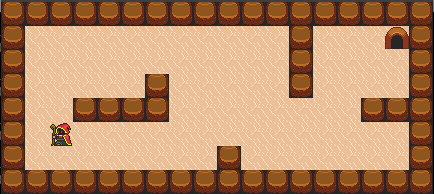
\includegraphics[width=0.5\textwidth]{./figures/experiment1}
\caption{Game environment for Evaluation 1}
\label{fig:experiment1}
\end{figure}
    
The purpose of the first evaluation is to highlight how ILP(RL) agent learns the hypotheses using inductive learning and executes an ASP planning.
The environment is a simple maze where the terminal state is located the right upper corner as shown in Figure \ref{fig:experiment1}.
The shortest time step between the agent's starting state and the terminal state is 18 steps, thus the maximum total reward the agent could gain is -8.

\subsection{Evaluation 1: Result}
\label{subsec:experiment1_result}

\begin{figure}[!htb]
\centering
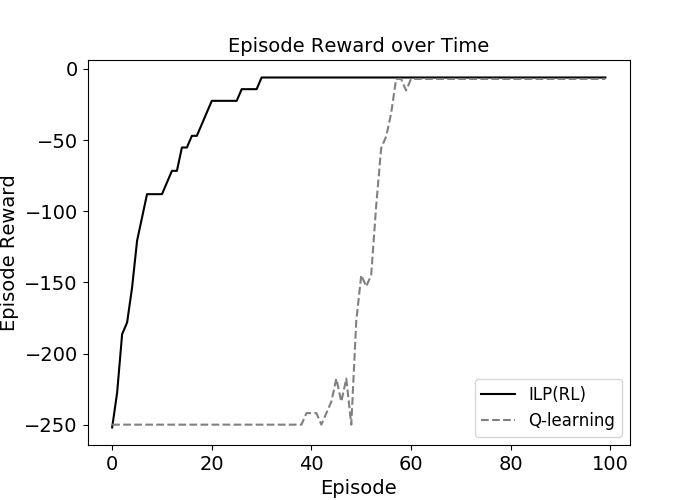
\includegraphics[width=0.7\textwidth]{./figures/experiment1_test}
\caption{Evaluation 1: optimal policy }
\label{experiment1_result}
\end{figure}

Figure \ref{experiment1_result} shows the performance of optimal policy.
ILP(RL) reaches the optimal policy faster than Q-learning: ILP(RL) reaches the optimal policy at before 40 episode, 
whereas Q-learning reaches the optimal policy at around 60 episode. ILP(RL) learns the optimal policy at an earlier episode because once the terminal state is found, the planning is always correct since there is only one way to reach the terminal state. The variations of the convergence to a optimal policy for ILP(RL) is dependent on how quickly the agent finds the terminal state. 
Since the exploration of ILP(RL) is based on $\epsilon$-greedy policy with the current ILP(RL), this result shows that there is a potential that a better exploration policy further improves the ILP(RL) learning.

The convergence of Q-learning for reaching an optimal policy is steeper than that of ILP(RL). This is because the state-action value functions are updated with the rate of $\alpha$, and the optimal policy for Q-learning is achieved when the optimal state-action value functions are achieved. By contrast, 
ILP(RL) gradually learns state transition of the environment using inductive learning and uses the background knowledge to accurately plan. 

Overall this result shows that ILP(RL) converges to the optimal policy faster than Q-learning in this simple scenario, achieving more data-efficient learning.

\lstinputlisting[
%   language = Prolog,
  caption  = {Hypotheses learnt in Evaluation 1},
  label = {list:experiment1_hypothesis}
]{experiment1_hypothesis.pl}

In addition to the data-efficient learning, what the agent has learnt with ILP(RL) is expressive.
Learnt hypotheses are shown in \ref{list:experiment1_hypothesis}, which are state transition for all directions, both when an adjacent state is a wall or not wall. The learnt state transitions are easy to understand for human users, and general in that they can be applied to a different similar environment.
The full learning task for this evaluation is in Appendix \ref{chap:learning_tasks_eval1}.

Next, we see how the agent learns the hypotheses over time. We plot part of the learning convergence for ILASP at episode 0 in Figure \ref{experiment1_ilasp}.
It converges to 1 after 200 episode, and shows that the agent learns the target hypotheses at the episode 0.
Since the two variables that the agent require to construct optimal answer set planning are the hypotheses and background knowledge, and the target hypotheses are learnt at episode 0, the convergence of finding an optimal policy for ILP(RL) is dependent on how quickly the agent finds a terminal state. 

\begin{figure}[!htb]
\centering
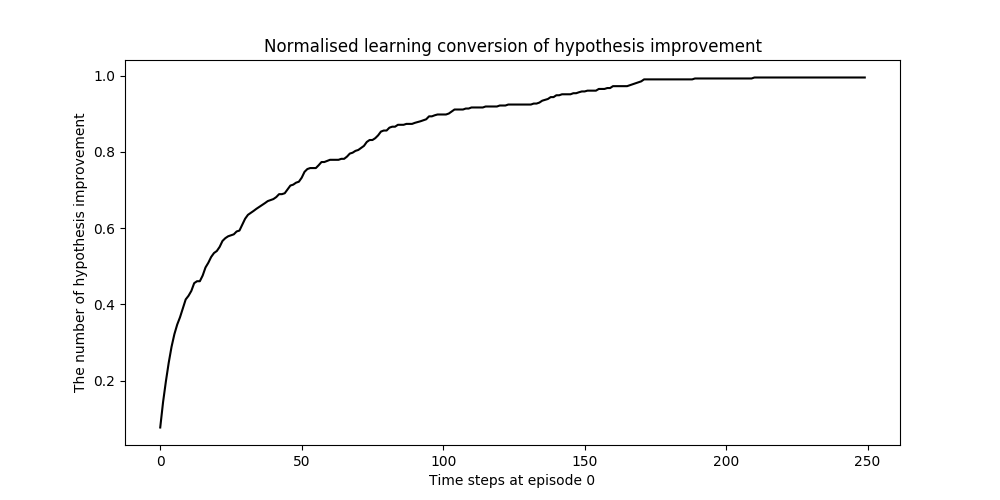
\includegraphics[width=0.7\textwidth]{./figures/experiment1_ilasp}
\caption{Normalised learning convergence by ILASP for experiment 1}
\label{experiment1_ilasp}
\end{figure}

Finally, we compare the runtime of two algorithms. 
The Figure \ref{exp1_runtime} shows that the runtime of ILP(RL) in the first few episodes is significantly high. 
This is due to the fact that ILP(RL) runs ILASP calls to learn the hypotheses at the beginning of episodes.
The Figure \ref{exp1_runtime} therefore highlights an issue that inductive learning is likely the bottleneck in terms of computational time.
This issue may not be critical in cases where the time of the time between the time steps is not an issue. If the performance is measured in terms of computation time rather than the number of iterations, 
ILP(RL) does not perform better than Q-learning. 
The average runtime of inductive learning is 5.58 seconds, and there are on average 12.83 times inductive learning per episode in this environment.
% RUNTIME FOR ILASP: 5.579039041812603
% ILASP RUNS TOTAL: 12.83 times
The ASP planning is not a bottleneck of ILP(RL), but still takes longer time than Q-learning, as can be observed by the divergence of cumulative runtime between the two algorithms. 
This experiment show that while ILP(RL) learns faster than Q-learning in terms of the number of episodes, it suffers from increasing computational time due to inductive learning as well as ASP planning.

\begin{figure}[!htb]
\centering
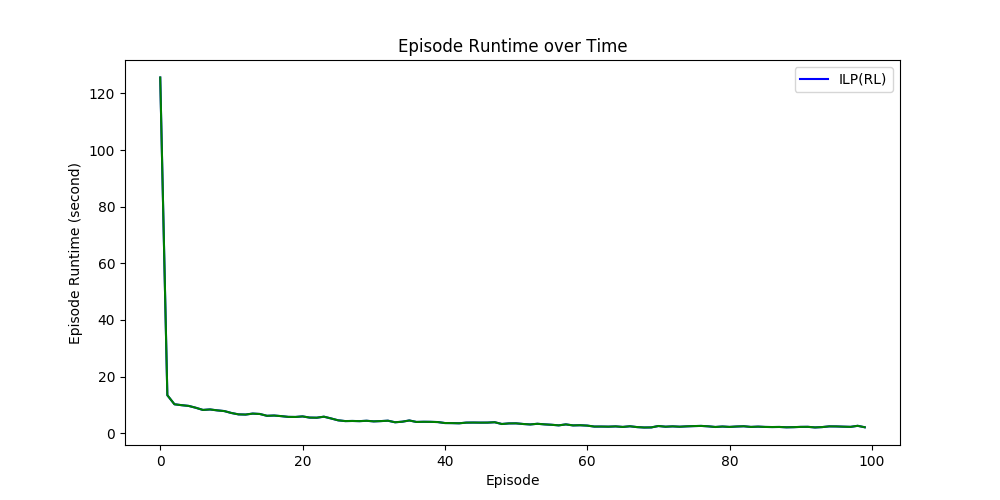
\includegraphics[width=0.7\textwidth]{./figures/experiment1_runtime}
\caption{Evaluation 1: runtime comparison}
\label{exp1_runtime}
\end{figure}

\subsection{Evaluation 2: Extended Baseline}
\label{subsec:experiement2_setup}

\begin{figure}[!htb]
\centering
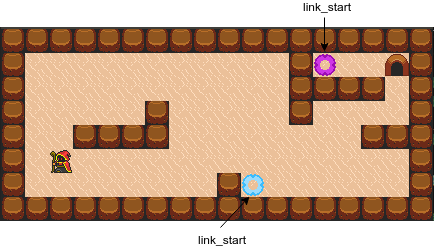
\includegraphics[width=0.5\textwidth]{./figures/experiment2_setup}
\caption{Game environment for Evaluation 2}
\label{experiment2}
\end{figure}
Evaluation 2 was conducted to see if the agent learns a teleport and finds an optimal path using the teleport. The environment is the same as Evaluation 1 except the presence of teleport link and three extra walls to surround the destination teleport.
In the environment shown in Figure \ref{experiment3},
there are two ways to reach the goal: using a floor path to reach the goal located on the top right corner, or using the teleport.
The environment is designed such that using the teleport is a shorter path and therefore gives a higher total reward.
Compared to Evaluation 1, two extra language biases are added as follows:
\begin{equation*}
\begin{split}
&\textsf{\#modeb(1, link\_start(var(cell)), (positive)).}\\
&\textsf{\#modeb(1, link\_dest(var(cell)), (positive)).}
\end{split}
\end{equation*}

\textsf{link\_start(var(cell))} is a state for departure of the teleport and \textsf{link\_dest(var(cell))} is the destination of the teleport. 
The teleport link is one-way: \textsf{link\_start} takes the agent to \textsf{link\_dest}, but \textsf{link\_dest} does not take the agent back to \textsf{link\_start}.
This extra types allows ILASP to learn additional hypotheses.
The full learning task for this evaluation is in Appendix \ref{chap:learning_tasks_eval2}.

Also \textsf{link\_start} and \textsf{link\_dest} need to be stored in background knowledge rather than as context dependent examples when the agent finds them, 
because ILP(RL) needs to generate exclusions regarding the teleport link behaviour.
The link locations need to be available for all positive examples so that ILASP correctly learns different a valid move for floor and teleport.

Because of the teleport link, the shortest path is 13 steps to reach the terminal state. Thus the maximum total reward that the agent could gain is -3.

\subsection{Evaluation 2: Result}
\label{subsec:experiment2_result}
    
\begin{figure}[!htb]
\centering
% 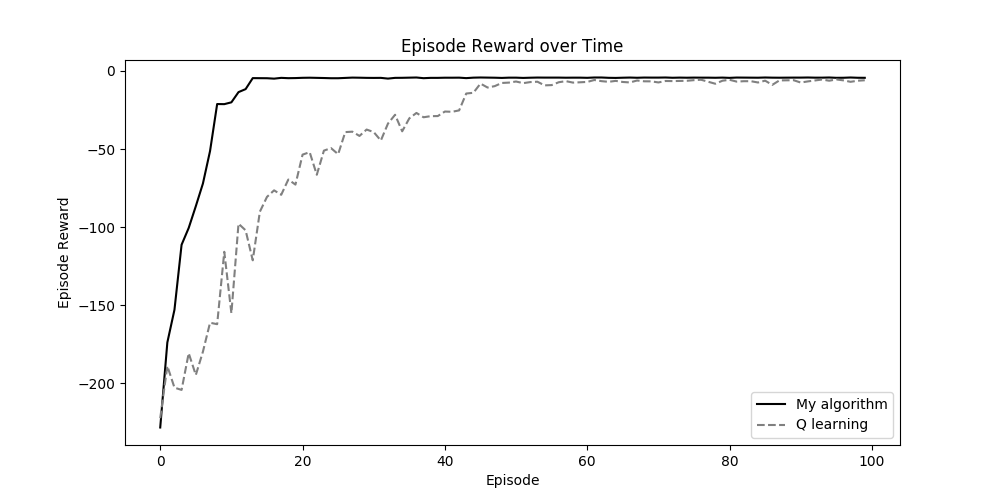
\includegraphics[width=0.55\textwidth]{./figures/experiment2_training}
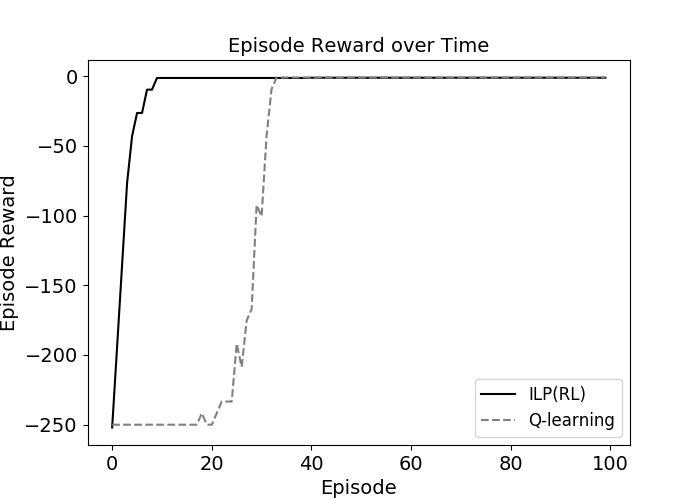
\includegraphics[width=0.7\textwidth]{./figures/experiment2_test}
\caption{Evaluation 2: optimal policy}
\label{experiment2_training}
\end{figure}

Similar to Evaluation 1, as shown in Figure \ref{experiment2_training}, ILP(RL) finds an optimal policy faster than Q-learning. Compared to the environment in Evaluation 1, ILP(RL) finds an optimal policy at earlier episode, because finding a terminal state is easier for ILP(RL) in this environment, since finding \textsf{link\_start} immediately leads the agent to the terminal state rather than having to go through a floor path to the upper right corner of the environment.
\newpage
\lstinputlisting[
  caption  = {Incomplete hypotheses for Evaluation 2},
  label = {experiment2_hypothesis_intermediate}
]{experiment2_hypothesis_intermediate.pl}

To highlight the inductive learning process of the new concept of teleport link, Listing \ref{experiment2_hypothesis_intermediate} is an intermediate incomplete hypotheses learnt by ILASP.
These hypotheses are generated just after the agent steps onto the \textsf{link\_start}. However, the first hypothesis in Listing \ref{experiment2_hypothesis_intermediate} states that
when \textsf{link\_dest} is available \textsf{state\_after} is true. Since \textsf{link\_dest} is available in background knowledge rather than context in the context dependent examples,
when solving for answer sets to generate a plan, it generates incorrect \textsf{state\_after} at every time step.

However, as shown in Definition \ref{def:ILPRL_exc}, these generated \textsf{state\_after} are all incorrect and therefore will be added to exclusions of the next positive example.
These exclusions will later refine hypotheses and the final complete hypotheses are shown in Listing \ref{list:exp2_final_hypotheses}.

\lstinputlisting[
  caption  = {Complete hypotheses for Evaluation 2},
  label = {list:exp2_final_hypotheses}
]{experiment2_hypothesis.pl}

Compared to the Evaluation 1, there are two new hypotheses due to the presence of the teleport links.
These learnt hypotheses are also applicable to an environment where there is no teleport links, such as the environment in Evaluation 1.
In this case, the first two hypotheses in Listing \ref{list:exp2_final_hypotheses} are never be used 
since the body predicates relating to link\_start(V0), link\_dest(V1) are never be satisfied.

\begin{figure}[!htb]
\centering
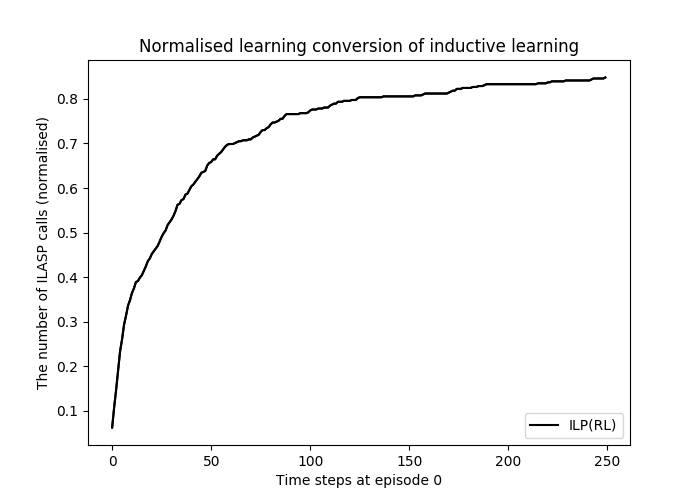
\includegraphics[width=0.7\textwidth]{./figures/experiment2_ilasp}
\caption{Normalised learning convergence by ILASP for Evaluation 2}
\label{experiment2_ilasp}
\end{figure}

Figure \ref{experiment2_ilasp} shows the learning convergence of inductive learning at episode 0.
Similar to Evaluation 1, most of ILASP calls occur at the beginning of the episode, as shown in Figure \ref{experiment2_runtime}.
The results of Evaluation 1 and 2 confirm that ILP(RL) learns state transition at the beginning of learning.
If the agent finds the teleport link state at a later episode, ILP(RL) refines the hypotheses by learning a new state transition regarding the teleport link.

\begin{figure}[!htb]
\centering
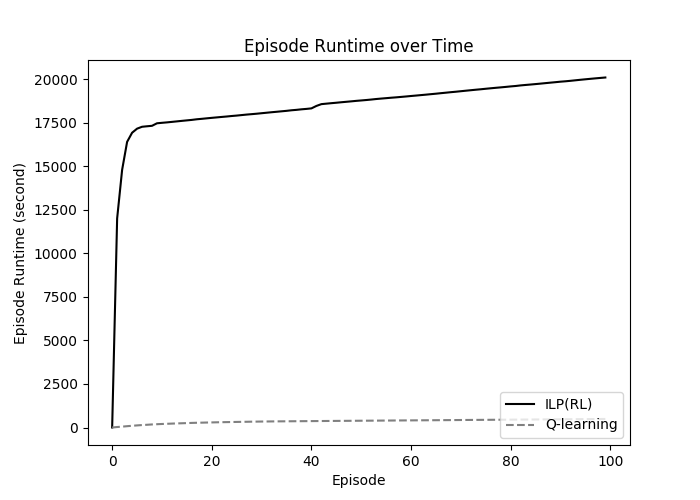
\includegraphics[width=0.7\textwidth]{./figures/experiment2_runtime}
\caption{Evaluation 2: runtime comparison}
\label{experiment2_runtime}
\end{figure}

Figure \ref{experiment2_runtime} shows the runtime of ILP(RL) and Q-learning in Evaluation 2. 
Despite the fact that the size of the environment is the same as Experiment 1,
there is a significant increase of runtime for ILP(RL) at the beginning of episode. 
This is because of the increase of search space in order for ILP(RL) to learn a new state transition.
The average runtime of inductive learning is 95.47 seconds, and there are on average 16.23 times inductive learning per episode.
% RUNTIME AVERAGE: 95.47274640401204
% RUNTIME COUNTS: 16.233333333333334
\begin{table}[!ht!b]
\centering
\begin{tabular}{lll}
\hline
Metrics            & Evaluation1    & Evaluation2      \\ \hline
Average ILASP runtime time (seconds)& 5.58        & 95.47       \\
The number of ILASP calls &  12.83      & 16.23      \\
Search space &  1690      & 32755       \\
\end{tabular}
\caption{Comparison of runtime, ILASP calls and search space between Evaluation 1 and 2}
\label{table:runtime_comparison}
\end{table}

To highlight the increase of runtime, Table \ref{table:runtime_comparison} summarises the comparison of runtime, ILASP calls and search space between Evaluation 1 and 2. 
Because of the two extra language biases for learning the teleport link, the search space in Evaluation 2 is significantly larger than that of Evaluation 1. This increase affects each ILASP call, resulting in much longer ILASP runtime in Evaluation 2. ILP(RL) calls ILASP an average of 3.4 more times in order to learn new hypotheses regarding the teleport link state.

While ILP(RL) still learns faster than Q-learning in terms of the number of iterations, 
the result of Experiment 2 shows that, the learning time per episode increases with respect to the size of search space, 
which corresponds to the number of state transition that the agent needs to learn in the environment.

\section{Transfer Learning Evaluation}
\label{sec:transfer_learning_evaluation}

\subsection{Evaluation 3: Transfer Learning}
\label{subsec:experiement3_setup}

\begin{figure}[!htb]
\centerline{

\includegraphics[width=0.5\textwidth]{./figures/experiment3_before}
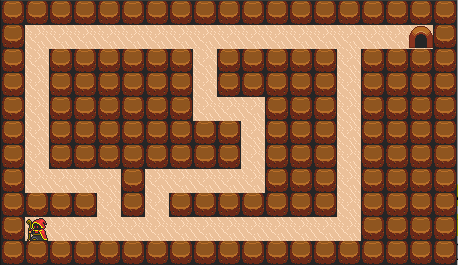
\includegraphics[width=0.5\textwidth]{./figures/experiment3_after}
}
\caption{Game environment for Evaluation 3: before (left) and after (right) transfer learning}
\label{experiment3_setup}
\end{figure}

In Evaluation 3, we investigate the possibilities of transfer learning between similar environments.
We trained the ILP(RL) agent using the environment on the left in Figure \ref{experiment3_setup}, 
and transfer the learnt hypotheses as well as context dependent examples to a new environment on the right in Figure \ref{experiment3_setup}. The terminal state is located at the same location, and there is an extra path in the environment on the right of Figure \ref{experiment3_setup}.

Context dependent examples are transferred to the new environment. This is because if there is a new hypothesis that the agent needs to learn in the new environment, 
ILP(RL) needs to refine the hypothesis using these transferred context dependent examples. Thus all the context dependent examples are also transferred as well as the learnt hypotheses. 

Background knowledge is not transferred since the wall locations are different in a new environment.
The agent therefore starts the exploration of the new environment with an empty background knowledge and gradually collects them over time.
The terminal state is the same as that in the first environment, but the shortest path to the goal is different between the two environments as new shorter path is introduced in the right environment in Figure \ref{experiment3_setup}.

In addition to Q-learning, we use three extra agents for comparison as follows. 

\begin{itemize}
    \item Agent(TL): The agent with transferred hypotheses, examples and also remembers the location of the terminal state.
    \item Agent(noTL)\textsubscript{Goal}: The agent with no transferred information, but knows the location of the terminal state.
    \item Agent(noTL)\textsubscript{noGoal}: The agent with no transferred information, including the location of the terminal state.
\end{itemize}

\lstinputlisting[
%   language = Prolog,
  caption  = {Hypotheses for Evaluation 3},
  label = {exp3_hypotheses}
]{experiment3_hypothesis.pl}

Listing \ref{exp3_hypotheses} is the hypotheses that is transferred to a new environment, which is acquired by training the agent in the environment once on the left of Figure \ref{experiment3_setup}.
The learnt hypotheses are the same hypotheses are that in Evaluation 1 shown in Listing \ref{list:experiment1_hypothesis} in the environment, they are a general concept that is applicable to any similar environments.

\subsection{Evaluation 3: Result}
\begin{figure}[!htb]
\centering
% 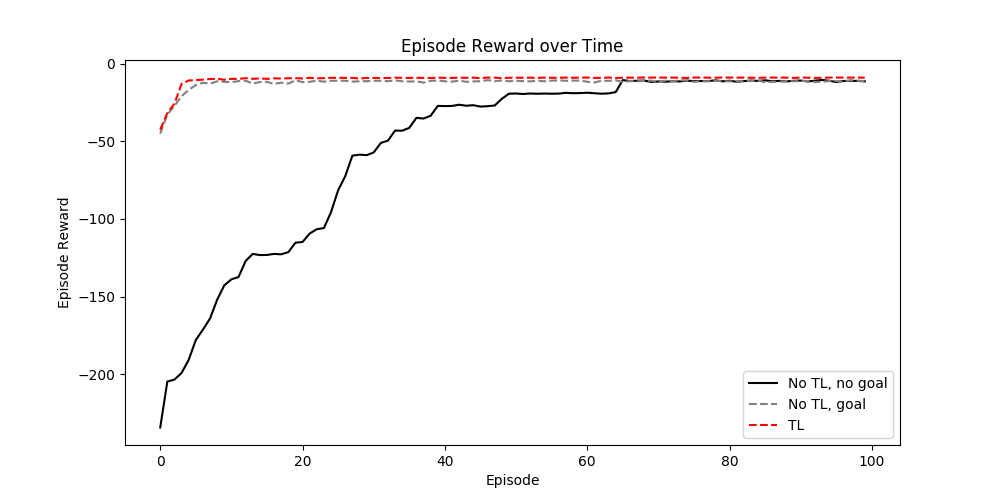
\includegraphics[width=0.55\textwidth]{./figures/experiment3_after_training}
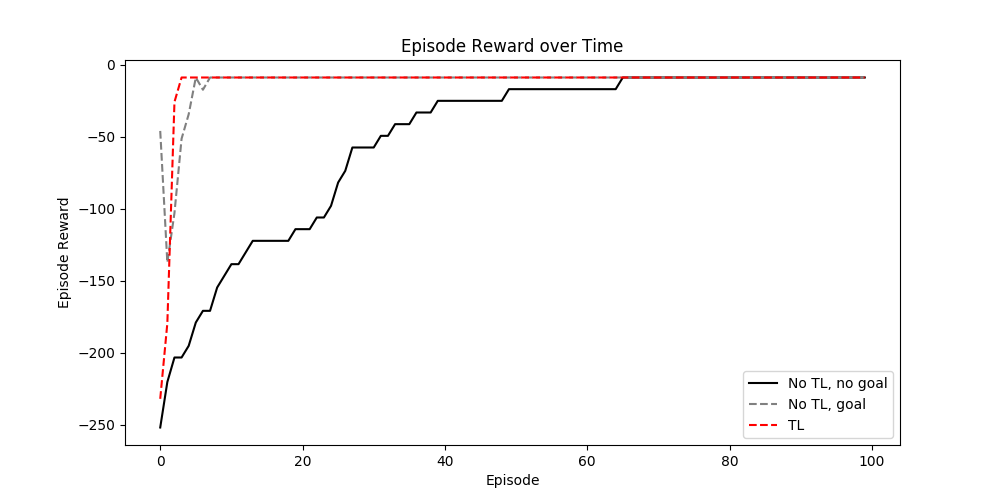
\includegraphics[width=0.7\textwidth]{./figures/experiment3_after_test}
\caption{Evaluation 3: optimal policy}
\label{experiment3_training}
\end{figure}

The result is shown in Figure \ref{experiment3_training}.
For Agent(TL), since the complete hypotheses are already known to the agent as well as the terminal state, the agent can do ASP planning from episode 0. There is no ILASP calls in the new environment since the transferred hypotheses are already the target hypotheses and cover all the examples the agent encounters in the new environment.
The only information required is background knowledge for the ASP planning, namely the locations of the walls, which are quickly acquired and reached the maximum total reward at the very beginning of episodes.

The next best agent in terms of convergence rate is Agent(noTL)\textsubscript{Goal}. Since the terminal state is known to the agent, 
the agent can do the planning from episode 0. However, the agent needs to learn the hypotheses. The reason that the convergence rate is almost the same as that of Agent(TL) is that, the ILP(RL) learns the complete hypotheses at very early episode, as observed in Evaluation 1 and 2. 
Thus there is no difference between Agent(TL) and Agent(noTL)\textsubscript{Goal} in terms of learning speed. 

What makes a difference for finding an optimal policy is whether the agent knows the terminal state, which can be seen by compering between Agent(noTL)\textsubscript{Goal} and Agent(noTL)\textsubscript{noGoal}.
The difference in terms of the iterations is that Agent(noTL)\textsubscript{noGoal} needs to find the terminal state first before starting the planning, which is a random exploration.

The capabilities of the transfer learning works especially when the terminal state is transferred, because the ASP planning of ILP(RL) depends on the terminal state. 
In addition, this evaluation further confirms that there is a promising potential for improving the exploration strategy to find the terminal state as soon as possible.

\subsection{Evaluation 4: Extended Transfer Learning}
\label{subsec:experiement4_setup}
\begin{figure}[!htb]
\centerline{

\includegraphics[width=0.5\textwidth]{./figures/experiment4_before}
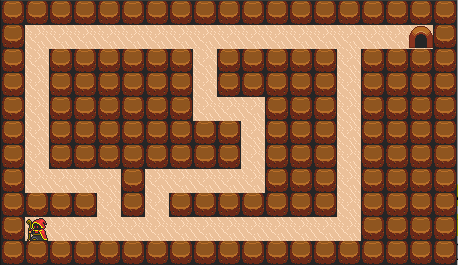
\includegraphics[width=0.5\textwidth]{./figures/experiment4_after}
}

\caption{Game environment for Evaluation 4: before (left) and after (right) transfer learning}
\label{experiment4_setup}
\end{figure}
In Evaluation 4, we trained ILP(RL) on the left in Figure \ref{experiment4_setup}, and transferred context dependent examples as well as the learnt hypotheses. The objective of this experiment is to see how the transferred agent learns a new state transition on top of the transferred hypotheses. In the new environment on the right of Figure \ref{experiment4_setup}, there is a teleport link and using the teleport is the shortest path to the terminal state. 
This is a new concept that did not exist in the trained environment and therefore the agent needs to learn it after the hypotheses are transferred.
The same as Evaluation 3, we use four different agents.

\subsection{Evaluation 4: Result}
\label{subsec:experiment_result_4}

\begin{figure}[!htb]
\centering
% 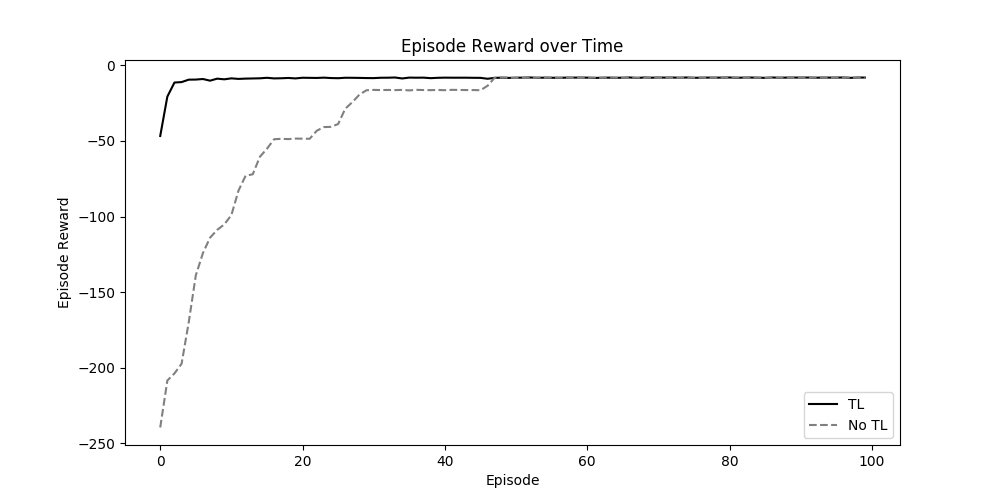
\includegraphics[width=0.55\textwidth]{./figures/experiment4_training}
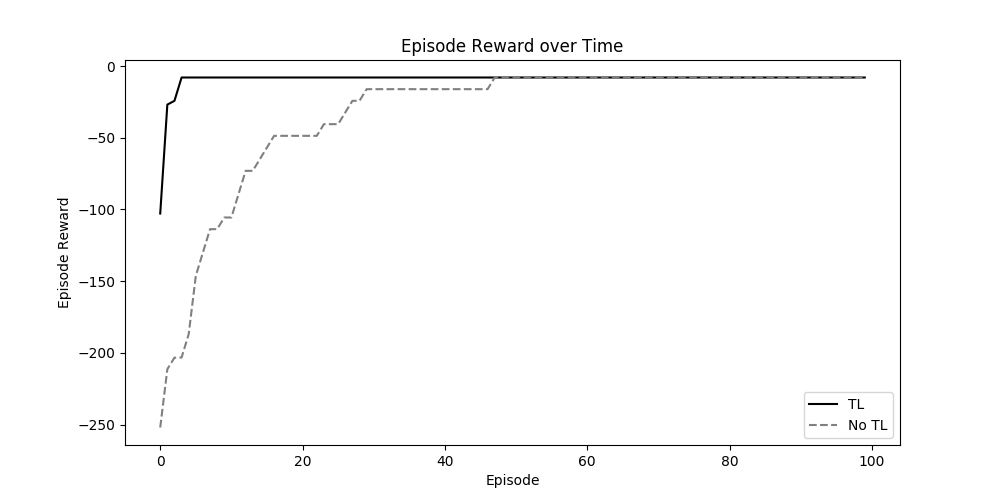
\includegraphics[width=0.7\textwidth]{./figures/experiment4_test}
\caption{Evaluation 4: optimal policy}
\label{experiment4_training_test}
\end{figure}

Figure \ref{experiment4_training_test} shows the results of optimal policy. 
Agent(TL) is able to successfully learn the new concept and quickly finds the optimal policy at the early episodes. Similar to Evaluation 3, Agent(notTL)\textsubscript{Goal} also quickly reaches the optimal policy,  
This experiment shows that the hypotheses is transferable even in cases where there is a new hypothesis the agent needs to learn in a new environment.

Also the difference of the state where the link is located does not cause any problems with ILP(RL) algorithm even when the positive examples in the previous environment are transferred. This is because information of ajacent walls are within the context of each example rather than background knowledge. This experiment shows the flexibility of context dependent examples in RL senarios.

The new hypotheses the agent learns are the same as that of Evaluation 2. The hypotheses regarding \textsf{link\_start} and \textsf{link\_dest} is what the Agent(TL) learnt in the new environment.

\section{Discussion}
\label{sec:discussion}

We evaluated the properties of ILP(RL) using simple maze environments. While the development of ILP(RL) is still in early stage and only a proof-of-concept, we observe both strengths as well as weakness of the current framework of ILP(RL). We summarise both of these in the following sections.

\subsection{Strengths of ILP(RL)}
As observed in the 4 evaluations, there are several advantages of ILP(RL) over Q-learning.

\begin{description}
\item[Faster learning of an optimal policy]
The ILP(RL) agent learns the general state transitions of the environment at the very early stage of learning, mostly at episode 0, and as soon as it finds the terminal state, is able to generate an ASP plan as a sequence of actions to find an optimal policy.
While this is a proof-of-concept approach, this way of RL is a new and the experiments show that this is a promising direction of the research.

\item[Transfer Learning]
Unlike existing RL algorithms, where it learns value functions or Q values, ILP(RL) learns a valid move as a hypotheses, which can be applied to similar but different environments.
We confirmed the possibility of transfer learning with the evaluations. Especially when the goal is known to the agent in Evaluation 3 and 4.
While this is a limited transfer learning since the terminal state is known in advance, this is still a useful transfer in cases where the terminal state is the same but the rest of the environment changes.
We also observed that the agent can learn a new hypothesis on top of the transferred hypotheses, which is very flexible in terms of applicability of the learnt hypotheses.

\item[Symbolic learning]
Since both the outcomes of ASP planning and inductive learning can be expressed in ASP syntax, the learning process as well as outcomes of ILP(RL) are easy to understand for human users, and the learnt hypotheses are very general state transitions of an environment.
\end{description} 

% The full hypotheses were learnt in the very early phase of learning and exploration phase. Thus with sufficient exploration, the model of the environment is correct
% and therefore it is able to find the optimal policy/path. 

% We show that ILP(RL) is able to solve a reduced MDP where the rewards are assumed to be associated with a sequence of actions planned as answer sets.
% Although this is a limited solution, there is a potential to expand it to solve full MDP as discussed in Further Research. 

\subsection{Limitations of the current framework}
\label{subsec:limitations}
Although the this first version of the ILP(RL) using inductive learning and ASP planning show potentials for a new way of solving RL problems, it is a proof-of-concept and there are a number of limitations with the current framework.
Some of these limitations are further elaborated in Further Research in Chapter \ref{sec:further_research}.

\begin{description}
\item[Runtime]
While we show that ILP(RL) converges to a optimal policy in terms of the number of episodes, the computational time is significantly longer than that of Q-learning due to the computation required for inductive learning with ILASP as well as ASP planning.
This limitation indicates that ILP(RL) may not be suitable in an environment where the runtime of learning is also a concern. ILP(RL) may also be unsuitable in an environment where there are moving objects based on time rather than time steps.

\item[Scalability issue for more complex environment]
ILP framework is known to be less scalable. The current framework is tested in a relatively simple environments, 
and proven to be work better than Q-learning in terms of learning an optimal policy by time. However, learning runtime of ILP(RL) in each time step is slower than that of Q-learning, which is worsen when there are more hypotheses that ILP(RL) needs to learn.
For example, as shown in Evaluation 1 and 2, adding two language bias significantly increased the runtime of the algorithm, since the search space grows significantly with respect to the language bias.
Whereas Q-learning updates value function regardless of whether there is a new concept such as teleport links, ILP(RL) needs to expands search space of hypotheses by adding more language bias. This is an important issue since many of RL research are focused on the development of RL algorithms in more complex environments.

Another question is the possibility of extending ILP(RL) to more realistic scenarios. RL works in more complex environments such as 3D or real physical environment, 
whereas the observations of an environment need to be expressed as ASP syntax for ILP(RL) to work.
\item[Requirements of assumptions]
ILP(RL) requires initial assumptions such as background knowledge or specification of language bias for search space. While most of existing reinforcement learning works in different kinds of environment without any pre-configuration, As shown in the Evaluation 2, it was necessary to add two extra modeb before learning starts.
Thus the current framework of ILP(RL) is unfeasible in cases where these learning concepts were unknown or difficult to define with language bias.

In addition, not only it needs search space, but also it is assumed that an agent knows the definition of adjacent state and is able to see the adjacent states. 
While this assumption may be reasonable in many cases, this is not common in traditional RL setting.

\item[solving limited MDP]
The current ILP(RL) framework does not make use of rewards for inductive learning and only uses the terminal state for ASP planning. While our evaluations were conducted in a simple environment and we assumed that there is only one reward for any states except a terminal state. As described in Section\ref{model_base_model_free_subsection}, other model-based RL methods learn a model of an environment, which tells the agent the reward and state transition functiosn. However, the current ILP(RL) only learns state transition and does not learn reward functions. In addition, some MDP problems contain no terminal state and instead there may be a different means to gain rewards. 
Since the current ILP(RL) is dependent on finding a terminal state for planning rather than maximising total rewards, 
the application of the current framework is limited to a particular type of MDP problem.

\end{description}  

Some of these issues are further discussed in Chapter \ref{conclusion}.

